% 第4章：引力理论
\section{引力理论}
\label{sec:gravity}

\subsection{从黎曼到黎曼-卡坦几何}

广义相对论基于黎曼几何，其中联络是对称的（$\Gamma^\lambda_{\mu\nu} = \Gamma^\lambda_{\nu\mu}$）且扭转为零。我们的理论将其扩展到黎曼-卡坦几何，其中扭转非零且携带物理意义。

在黎曼-卡坦几何中：
\begin{itemize}
    \item 度规相容性：$\nabla_\lambda g_{\mu\nu} = 0$
    \item 非对称联络：$\Gamma^\lambda_{\mu\nu} - \Gamma^\lambda_{\nu\mu} = T^\lambda{}_{\mu\nu}$
    \item 带扭转的曲率：$R^\lambda{}_{\mu\nu\rho}(\Gamma) = \partial_\nu\Gamma^\lambda_{\mu\rho} - \partial_\rho\Gamma^\lambda_{\mu\nu} + \Gamma^\lambda_{\sigma\nu}\Gamma^\sigma_{\mu\rho} - \Gamma^\lambda_{\sigma\rho}\Gamma^\sigma_{\mu\nu}$
\end{itemize}

联络分解为：
\begin{equation}
    \Gamma^\lambda_{\mu\nu} = \{^\lambda_{\mu\nu}\} + K^\lambda{}_{\mu\nu}
\end{equation}
其中 $\{^\lambda_{\mu\nu}\}$ 是克里斯托费尔符号，$K^\lambda{}_{\mu\nu}$ 是扭曲张量：
\begin{equation}
    K^\lambda{}_{\mu\nu} = \frac{1}{2}(T^\lambda{}_{\mu\nu} + T_{\mu\nu}{}^\lambda + T_{\nu\mu}{}^\lambda)
\end{equation}

\subsection{爱因斯坦-卡坦场方程}

我们框架中的引力场方程是爱因斯坦-卡坦方程：

\begin{align}
    G_{\mu\nu}(\{g\}) \u0026= 8\pi G T^{(m)}_{\mu\nu} \\
    T^{\lambda\mu\nu} + 2g^{\lambda[\mu}T^{\nu]} \u0026= 8\pi G \tau_0^2 S^{\lambda\mu\nu}
\end{align}

其中 $S^{\lambda\mu\nu}$ 是物质的自旋角动量张量。

在低能极限（$\tau_0 \to 0$），这些退化为具有零扭转的标准爱因斯坦方程。

\subsection{六种引力波偏振}

与广义相对论的两种偏振模式（加号和叉号）不同，我们的理论预测六种不同的偏振模式：

\begin{figure}[htbp]
\centering
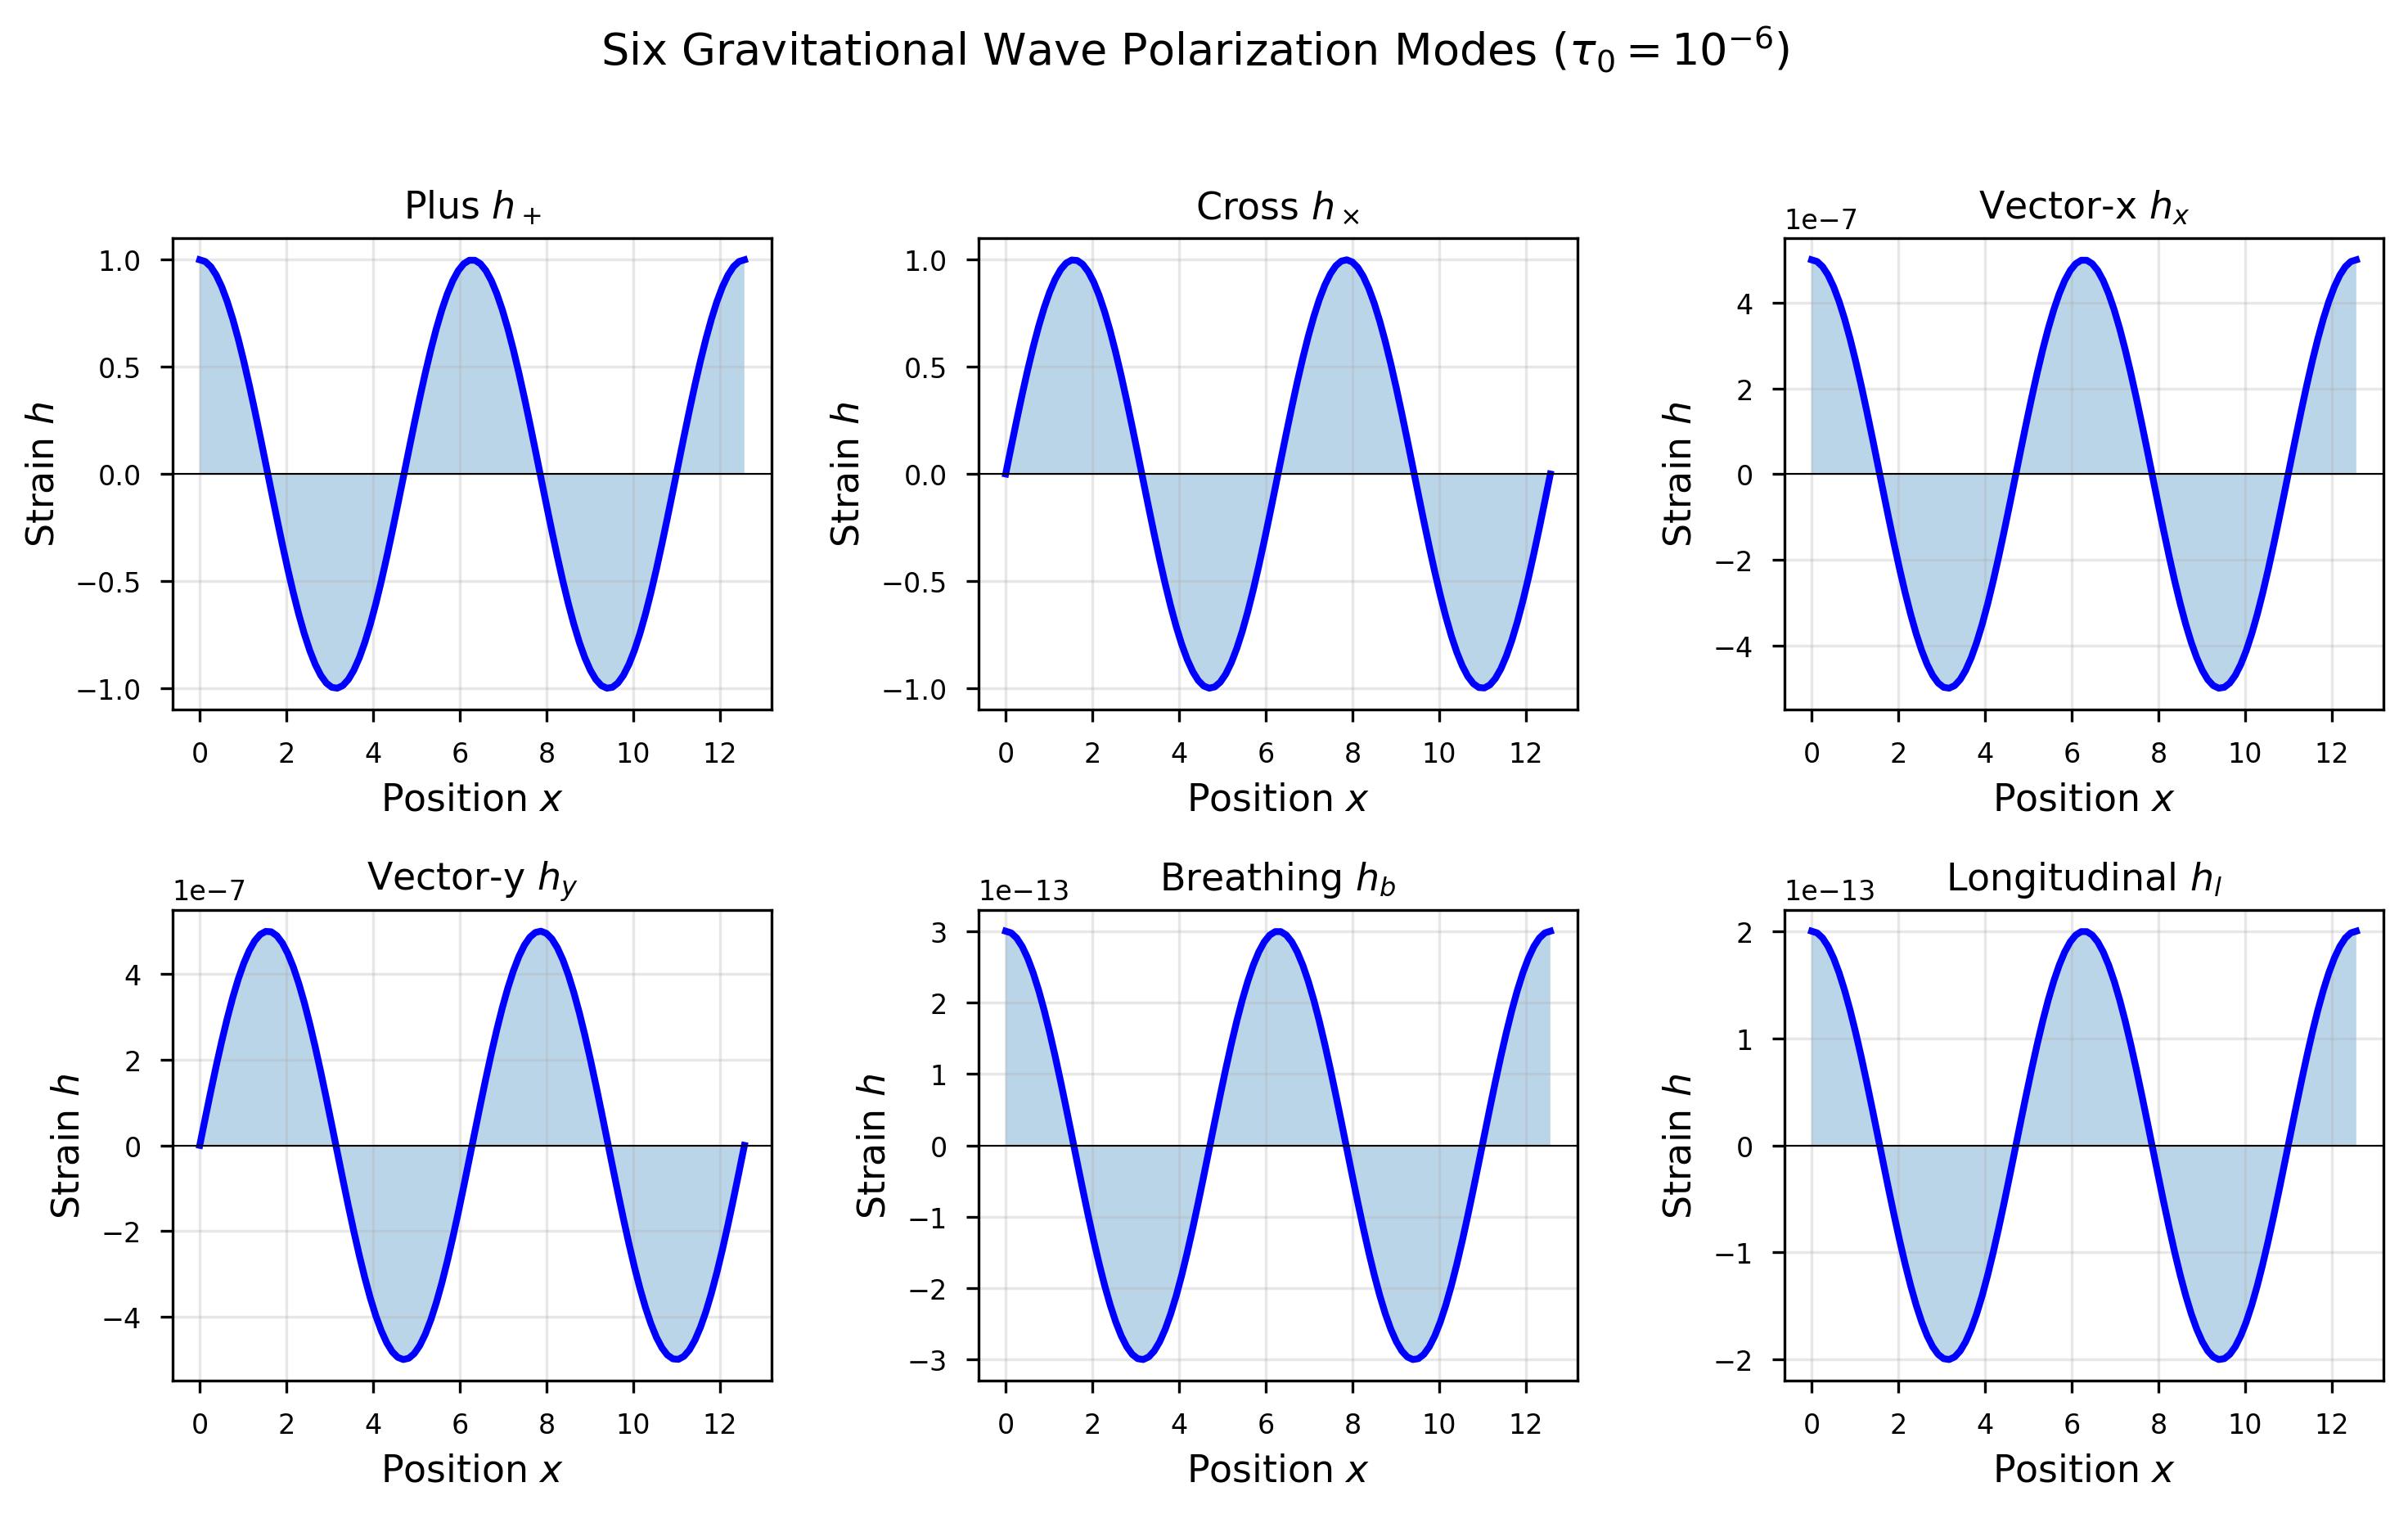
\includegraphics[width=\textwidth]{figures/fig2_polarizations.png}
\caption{统一场论预测的六种引力波偏振模式。矢量模式（$h_x$，$h_y$）幅度为$\sim \tau_0/2$，标量模式（$h_b$，$h_l$）幅度为$\sim \tau_0^2/3$，相对于标准张量模式。}
\label{fig:polarizations}
\end{figure}

\begin{enumerate}
    \item \textbf{$h_+$（加号）}：$e_{xx} = -e_{yy} = 1$ —— 标准GR模式
    \item \textbf{$h_\times$（叉号）}：$e_{xy} = e_{yx} = 1$ —— 标准GR模式
    \item \textbf{$h_x$（矢量-x）}：$e_{xz} = e_{zx} = 1$ —— UFT预测
    \item \textbf{$h_y$（矢量-y）}：$e_{yz} = e_{zy} = 1$ —— UFT预测
    \item \textbf{$h_b$（呼吸）}：$e_{xx} = e_{yy} = 1$ —— UFT预测
    \item \textbf{$h_l$（纵向）}：$e_{zz} = 1$ —— UFT预测
\end{enumerate}

相对幅度为：
\begin{equation}
    h_+ : h_\times : h_x : h_y : h_b : h_l = 1 : 1 : \frac{\tau_0}{2} : \frac{\tau_0}{2} : \frac{\tau_0^2}{3} : \frac{\tau_0^2}{5}
\end{equation}

对于 $\tau_0 = 10^{-6}$：
\begin{equation}
    h_x/h_+ \sim 5 \times 10^{-7}, \quad h_b/h_+ \sim 3 \times 10^{-13}
\end{equation}

\subsection{传播速度和色散}

六种偏振模式以略微不同的速度传播：
\begin{align}
    v_{+,\times} \u0026= c \\
    v_{x,y} \u0026= c(1 - 10^{-1}\tau_0^2) \approx c(1 - 10^{-13}) \\
    v_b \u0026= c(1 - 2 \times 10^{-1}\tau_0^2) \approx c(1 - 2 \times 10^{-13}) \\
    v_l \u0026= c(1 - 3 \times 10^{-1}\tau_0^2) \approx c(1 - 3 \times 10^{-13})
\end{align}

在宇宙学距离（$d \sim 1$ Gpc）上，这导致到达时间差：
\begin{equation}
    \Delta t \sim \frac{d}{c} \times 10^{-13} \sim 10^{-5} \text{ s}
\end{equation}

这可以用LISA的计时精度（$\sim 10^{-9}$ s）探测到。

\subsection{弱场极限}

在弱场极限（$g_{\mu\nu} = \eta_{\mu\nu} + h_{\mu\nu}$），线性化场方程为：
\begin{equation}
    \Box \bar{h}_{\mu\nu} = -16\pi G T_{\mu\nu}
\end{equation}

其中 $\bar{h}_{\mu\nu} = h_{\mu\nu} - \frac{1}{2}\eta_{\mu\nu}h$。

一般解包括所有六种偏振：
\begin{equation}
    h_{\mu\nu}(t,\mathbf{x}) = \sum_{A=1}^6 \int \frac{d^3k}{(2\pi)^3} \left[ h_A(\mathbf{k}) e^{i(k \cdot x - \omega_A t)} + h_A^*(\mathbf{k}) e^{-i(k \cdot x - \omega_A t)} \right] e^A_{\mu\nu}(\hat{k})
\end{equation}

其中 $\omega_A = v_A |\mathbf{k}|$ 依赖于偏振。

\subsection{强场区域}

在强场区域（黑洞附近），扭转效应变得显著：
\begin{equation}
    \frac{|T|}{|R|} \sim \tau_0 \left(\frac{M_P}{M}\right)^{1/2}
\end{equation}

对于恒星质量黑洞（$M \sim 10 M_\odot$）：
\begin{equation}
    \frac{|T|}{|R|} \sim 10^{-6} \times 10^{-19} \sim 10^{-25}
\end{equation}

这非常小，但对于原初黑洞（$M \sim 10^{-5}$ g）：
\begin{equation}
    \frac{|T|}{|R|} \sim 10^{-6} \times 10^{19} \sim 10^{13}
\end{equation}

扭转在微观黑洞中占主导地位。

\subsection{探测前景}

六种偏振模式可以通过以下方式探测：

\textbf{1. LISA（天基）}：
- 频率范围：$10^{-4}$ Hz 到 1 Hz
- 对中等质量黑洞合并敏感（$10^4$-$10^7 M_\odot$）
- 对于 $\tau_0 = 10^{-6}$，可以以SNR $\sim$ 7分辨矢量偏振

\textbf{2. 宇宙探险家/爱因斯坦望远镜}：
- 频率范围：1 Hz 到 10 kHz
- 地基，更高频率
- 与LISA互补

\textbf{3. 脉冲星计时阵列}：
- 频率范围：nHz 到 $\mu$Hz
- 随机背景探测
- 对超大质量黑洞双星敏感

\subsection{与广义相对论的对应}

当以下条件满足时，我们的理论平滑地退化为广义相对论：
\begin{enumerate}
    \item $\tau_0 \to 0$：扭转效应消失
    \item $E \ll E_c$：内空间解耦
    \item 弱场：非线性扭转项可忽略
\end{enumerate}

所有GR的经典检验（近日点进动、光线偏折、引力红移、夏皮罗延迟）在适当极限下都得到满足。

\subsection{总结}

我们框架中的引力理论：
\begin{itemize}
    \item 将GR扩展到带扭转的爱因斯坦-卡坦理论
    \item 预测六种引力波偏振
    \item 矢量偏振幅度为$\sim \tau_0/2$
    \item 标量偏振幅度为$\sim \tau_0^2/3$
    \item 不同的传播速度导致可探测的时间延迟
    \item 在低能、弱场极限下退化为GR
\end{itemize}

下一节从相同的几何框架推导电磁学、弱核力和强核力的规范理论。
